\documentclass[border=0.5mm,tikz]{standalone}

\usepackage{ifthen}
\usepackage{cmap}
% \usepackage[defaultsans]{droidsans}
% \renewcommand*\familydefault{\sfdefault} %% Only if the base font of the document is to be typewriter style
\usepackage[T2A]{fontenc}
\usepackage[utf8x]{inputenc}
\usepackage{amsmath,amssymb}
\usepackage{esdiff,esint}


\usepackage{pgfplots}
\usetikzlibrary{shapes, arrows}
% \pgfplotsset{compat=1.10}
\pgfplotsset{compat=newest}
\usepgfplotslibrary{fillbetween}
\usetikzlibrary{patterns,calc}
\usepackage[outline]{contour}

\usetikzlibrary{quotes,angles}
% Example:
%   \lineann[1]{30}{2}{$L_1$}
% \newcommand{\lineann}[4][0.5]{%
%     \begin{scope}[rotate=#2, blue,inner sep=2pt]
%         \draw[dashed, blue!40] (0,0) -- +(0,#1)
%             node [coordinate, near end] (a) {};
%         \draw[dashed, blue!40] (#3,0) -- +(0,#1)
%             node [coordinate, near end] (b) {};
%         \draw[|<->|] (a) -- node[fill=white] {#4} (b);
%     \end{scope}
% }
\begin{document}

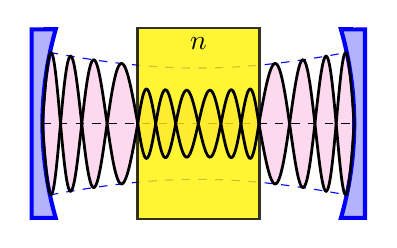
\begin{tikzpicture}
\xdef\len{8}

\xdef\wo{3}
\xdef\coeff{0.9}
\xdef\Z{\len}
\xdef\Shift{10}
\xdef\AngleShift{4}
\pgfmathparse{\len+1.2}\let\xmaxx\pgfmathresult
\pgfmathparse{\wo*sqrt(1+(\coeff*\Z/\wo^2)^2)}\let\H\pgfmathresult
\pgfmathparse{atan((\H)/(\Z+\Shift))+\AngleShift}\let\angle\pgfmathresult

\pgfmathparse{tan(\angle)*(\Z+\Shift)+0}\let\ymaxx
% l длина
% n полупериодов
% lena длина полпериода в координатах рисунка
% n/l*180*x
\pgfmathresult

\pgfmathparse{sqrt((\Z+\Shift)^2+\H^2)}\let\Rad\pgfmathresult

\tikzset{
    gaussfill/.style={
        fill=magenta, opacity=0,
    },
    gaussdraw/.style={
        blue, dashed
    },    
    sin/.style={
        black, line width=1pt,
    },
    sinfill/.style={
        fill=magenta, opacity=0.15,
    },
    mirror/.style={
        blue, line width=1.5pt,
        fill=blue!30
    },
    diel/.style={
       % pattern=north east lines,
       draw=black, line width=1pt, fill=yellow, opacity=0.8,
    },
}


\begin{axis}[axis lines=middle,
            xlabel={$z$},
            ylabel={$w(z)$},
            hide axis,
            scale=0.8,
            width=7cm,
            height=5cm,
            % enlargelimits,
            unit vector ratio*=1 1 1,
            ytick=\empty,
            xtick=\empty,
            ymin=-\ymaxx,
            % ymax={\ymaxx+2.5},
            ymax={\ymaxx},
            xmin=-{\xmaxx},
            xmax={\xmaxx},
            disabledatascaling,
            % domain=-2:2, 
            % restrict y to domain=-2:2,
            % xtick={1,4},
            % xticklabels={a,b}
            ]


\contourlength{0.6mm};
\addplot[name path=A,gaussdraw,domain={-\len:\len},samples=100] {\wo*sqrt(1+(\coeff*x/\wo^2)^2)} node[pos=.8, above]{};


\addplot[name path=B,gaussdraw,domain={-\len:\len},samples=100] {-\wo*sqrt(1+(\coeff*x/\wo^2)^2)} node[pos=.8, above]{};

\addplot[gaussfill]fill between[of=A and B, soft clip={domain=-\len:\len}];


\begin{scope}[xscale=-1]
\draw[draw=none] (0,0) coordinate (0) -- (\Z,\H) coordinate (A);
\draw[draw=none] (0,0) -- (\Z,-\H) coordinate (B);
\path[mirror,draw=none,opacity=0,name path=C]([shift=(-\angle:\Rad)]-\Shift,0) arc (-\angle:\angle:\Rad);
\draw[mirror] ([shift=(-\angle:\Rad)]-\Shift,0) coordinate (2) arc (-\angle:\angle:\Rad) -- ++ (1.3,0) -- ($(2)+(1.3,0)$) -- (2) -- cycle;
\path[name path=D] (A) -- (B);
\addplot[gaussfill]fill between[of=C and D];
\end{scope}

\begin{scope}[xscale=1]
\draw[draw=none] (0,0) coordinate (0) -- (\Z,\H) coordinate (A);
\draw[draw=none] (0,0) -- (\Z,-\H) coordinate (B);
\path[mirror,draw=none,opacity=0,name path=C]([shift=(-\angle:\Rad)]-\Shift,0) arc (-\angle:\angle:\Rad);
\draw[mirror] ([shift=(-\angle:\Rad)]-\Shift,0) coordinate (2) arc (-\angle:\angle:\Rad) -- ++ (1.3,0) -- ($(2)+(1.3,0)$) -- (2) -- cycle;
\path[name path=D] (A) -- (B);
\addplot[gaussfill]fill between[of=C and D];
\end{scope}

\draw[dashed] (-\Rad+\Shift,0) -- (\Rad-\Shift,0);

\xdef\n{13}
\xdef\inside{3}
\xdef\scr{0.6} % сжатие по вертикали в диэлектрике
\pgfmathparse{\n/(\Rad-\Shift)/2*180}\let\omegga\pgfmathresult
\pgfmathparse{1/(\n/(\Rad-\Shift)/2)}\let\lena\pgfmathresult
% l длина
% n полупериодов
% lena длина полпериода в координатах рисунка
% n/l*180*x
\ifthenelse{\isodd{\n}}%
    {%нечет
        \xdef\phhi{90}
    }%чет
    {  
        \xdef\phhi{0}
        % \xdef\lefft{\lena}
    }%
        \xdef\lefft{\lena*\inside/2}

\pgfmathparse{\Rad-\Shift}\let\mirror\pgfmathresult
% \draw[diel] (-\lefft,-\ymaxx) rectangle (\lefft,\ymaxx) ;
\xdef\leff{3.28}
\draw[diel] (-\leff,-\ymaxx) rectangle (\leff,\ymaxx) ;

\draw (0,\ymaxx) node[below] {$n$};
\draw (0,-\ymaxx) node[below] {$m=\inside$};
% \draw (0,0) node {\ymaxx};

\draw[dashed, blue!40] (-\mirror,\ymaxx) -- +(0,2.5)
            node [coordinate, near end] (a) {};
        \draw[dashed, blue!40] (\mirror,\ymaxx) -- +(0,2.5)
            node [coordinate, near end] (b) {};
        \draw[|<->|] (a) -- node[fill=white] {$L$} (b);

\xdef\p{20.55}
\xdef\N{2}
\addplot[name path=psinus1,sin,domain={-\Rad+\Shift:\Rad-\Shift},samples=400] {\wo*sqrt(1+(\coeff*x/\wo^2)^2)*sin((abs(x)<\leff?\omegga*\N:\omegga)*x/(1/\p*(abs(x)-\p))/2+\phhi+(abs(x)<\leff?90:0))*(abs(x)<\leff?\scr:1)} node[pos=.8, above]{};

\addplot[name path=psinus2,sin,domain={-\Rad+\Shift:\Rad-\Shift},samples=400] {-\wo*sqrt(1+(\coeff*x/\wo^2)^2)*sin((abs(x)<\leff?\omegga*\N:\omegga)*x/(1/\p*(abs(x)-\p))/2+\phhi+(abs(x)<\leff?90:0))*(abs(x)<\leff?\scr:1)} node[pos=.8, above]{};  

\addplot[sinfill] fill between [of=psinus1 and psinus2, soft clip={domain=-\Rad+\Shift:\Rad-\Shift}];



\end{axis}
\end{tikzpicture}
\end{document}

% \draw (0,0) pic[draw=black, <->,>=latex', angle eccentricity=1.2, angle radius=1cm]
    % {angle=B--0--A};

% \draw (2.3,0) node[right,fill=white,rounded corners=2pt,inner sep=1pt,fill opacity=0.8] {\contour{white}{$2\vartheta=\frac{2\lambda}{\pi w_0}$}};

% \draw (2.3,0) node[right,rounded corners=2pt,inner sep=1pt,] {{$2\vartheta=\frac{2\lambda}{\pi w_0}$}};
% \pgfmathparse{1*(\Z*(1+(\wo^2/(\coeff*\Z))^2))}\let\Radius\pgfmathresult
% \xdef\Radius{2}
% \xdef\angle{15}
% \pgfmathparse{6-\Radius}\let\coo\pgfmathresult
%(-\angle:\angle:\Radius);
% \draw[dashed] ({-1},{exp(-1)}) -- ({-2.5},{exp(-1)});



% \draw[|<->|,>=latex'] (-0.9,-\wo) -- node[pos=0.5] {\contour{white}{$2w_0$}} (-0.9,\wo);


% \draw[|<->|,>=latex'] ({-2.4},{0}) -- node[pos=0.55] {\contour{white}{$E_0/e$}} ({-2.4},{exp(-1)});

% \draw[|<->|,>=latex'] ({2.4},{0}) -- node[pos=0.5] {\contour{white}{$E_0$}} ({2.4},{1});

% \draw[dashed] ({2.5},{1}) -- ({0},{1});
% \addplot[name path=B,blue,domain={-\To:-\From},samples=100] {1/x} node[pos=.8, above]{};

% \addplot[pattern=north east lines, pattern color=black!50]fill between[of=B and xmin, soft clip={domain=-\To:-\From}];

% \addplot[pattern=north east lines, pattern color=black!50]fill between[of=A and xmax, soft clip={domain=\From:\To}];

% \addplot[pattern=north east lines, pattern color=black!50]fill between[of=axisx and xmin, soft clip={domain=0:\To}];

% \addplot[pattern=north east lines, pattern color=black!50]fill between[of=axisx and xmax, soft clip={domain=-\To:0}];

% \draw [densely dashed, opacity=0.3] (-2,-2) -- (2,2);

% \draw[dashed] (-1,0) 
%       -- (-1,-1)
%       -- (0,-1);

% \draw[dashed] (1,0) 
%       -- (1,1)
%       -- (0,1);


% % \contourlength{1cm}; 


% \coordinate (parallel)  at (2,1.5);
% \coordinate (ust)  at (-1.5,1);
% \coordinate (conc)  at (-2.1,-1.5);
% \coordinate (conf)  at (1.5,-1);

% \xdef\Scale{1}
% % \contour{white}{}
% \node[scale=1.1,align=center] at (ust)  {\contour{white}{Условие устойчивости:}\\\contour{white}{$0<g_1g_2<1$}\\\\\contour{white}{где}\\\\\contour{white}{$g_1=1-\frac{d}{R_1},\quad g_2=1-\frac{d}{R_2}$}};


% \draw (parallel) node[scale=\Scale,align=center]  {\contour{white}{Плоские зеркала}\\\contour{white}{($R_1=R_2=\infty$)}}
% node[inner sep=0pt, yshift=-1.5em, below] at (parallel)
%     {
\includegraphics[width=7em]{parallel}};


% \draw (conc) node[scale=\Scale,align=center]  {\contour{white}{Концентрические}\\\contour{white}{зеркала}\\\contour{white}{($R_1=R_2=d/2$)}} node[above,inner sep=0pt,yshift=1.7em] 
%     {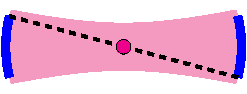
\includegraphics[width=7em]{conc}};



% \draw (conf) node[inner sep=0pt,above]
%     {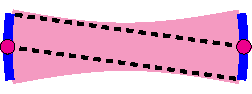
\includegraphics[width=7em]{conf}} node [below, align=center,scale=\Scale] {\contour{white}{Конфокальные}\\\contour{white}{зеркала}\\\contour{white}{($R_1=R_2=d$)}};
% % \node[coordinate,pin=30:{$A$}] at (3.8,3){};

% \coordinate (A) at (0.7,-0.75);
% \coordinate (0) at (0,0);
% % \draw (A) -- (0);
% \path[draw] (A) edge [out=180, in=-80,->, thick, >=latex] (0);

% \draw[fill=magenta] (0,0) circle (2pt);

% \draw[fill=magenta] (1,1) circle (2pt) node[left, yshift=-1em, scale=0.8]{\contour{white}{$(1,1)$}};

% \draw[fill=magenta] (-1,-1) circle (2pt) node[right, yshift=1em, scale=0.8]{\contour{white}{$(-1,-1)$}};

% \draw[magenta, line width=1.5pt,] (1)--($(1)+(0.25,0)$)--($(2)+(0.25,0)$) -- (2);
\end{axis}
\end{tikzpicture}
\end{document}